\chapter{Putting it all together}\label{ch:putting-it-all-together}

As the name of this chapter suggests, we now put the knowledge from the previous chapters together.
We build the Abstract Interpretation framework for data manipulation programs.
It involves defining the concrete and abstract lattice and the Galois connection between.

Since we are mostly focusing on Pandas in Python, we assume Python environment with Pandas, specifically:

\begin{itemize}
    \item Python syntax
    \item Standard Python data types - int, float, string, list, dictionary, tuple
    \item Pandas is imported via \verb|import pandas as pd| statement
\end{itemize}

We also assume, unlike the Pandas, that Series are homogenous and Dataframes have homogenous columns.
This also implies that each column of a Dataframe has an associated type.

\begin{defn}
    Let Df be a Dataframe and Sr a Series.
    We assume the following operations for accessing metadata about the two structures:

    \verb|columns(Df) = { Sr1 .. Srn }| \\

    \verb|type(Sr) - returns type| \\

    \verb|name(Sr) - returns name| \\
\end{defn}

Given these assumptions, we can define a Dataframe Structure:

\begin{defn}[Dataframe Structure]
    For a Dataframe $Df$, its \textbf{Dataframe} Structure is $DS(Df) = \{ (name(Sr), type(Sr)) | Sr \in columns(Df) \}$
\end{defn}

Also, we define a Series Structure:

\begin{defn}[Series Structure]
    For a Series $Sr$, its \textbf{Series Structure} is $SS(Sr) = (name(Sr), type(Sr))$
\end{defn}


\section{The concrete lattice}

The concrete lattice should correspond with the reality.
Since the variables of our program are Dataframes and Series, we can imagine the set of all possible Dataframes and
Series (with every finite number of rows/columns and all possible values).
Then we define the concrete lattice as the power set of this set with the inclusion being the ordering. % todo chaotic
To formalize this:

\begin{defn}[The concrete lattice]

    Let
    \begin{gather*}
        C = \{\forall df \: Dataframe: df\} \cup \{\forall sr \: Series: sr\}
    \end{gather*}
    Then the concrete lattice is $L_c = (\powerset{C}, \subseteq)$
\end{defn}


\section{The abstract lattice}

The abstract lattice can be chosen by us depending on how much we want to abstract the values.
We would like the abstraction to be actually useful in practice.
What does this mean?
In the Abstract Interpretation, whenever we should get a value from the user, we approximate it by the supremum of our
lattice.
This is usually done when we do not know anything about the input, since it is the most precise approximation that is
still sound.
However, we can do something smarter.
We will create and use the assumption that whenever the user inputs a Dataframe, the Column Structure of that Dataframe
is known in advance.
This is not a very strong assumption in practice given the fact that the structure of the dataframe is usually known
during the process of writing the program anyway - otherwise we would not be able to write the program at all.

So the abstract lattice consists of the Dataframe Structures and Series Structures.
We take the set of all possible Dataframe Structures and Series Structures.
Then the abstract lattice is the power set of that set with the inclusion being the ordering.
We again formalize this:

\begin{defn}[The abstract lattice]

    Let
    \[A = \{\forall df\: Dataframe: DS(df)\} \cup \{\forall sr \: Series: SS(sr)\}\].
    Then the abstract lattice is $L_a = (\powerset{A}, \subseteq)$
\end{defn}

\section{The Galois Connection}

To create a Galois Connection we need an abstraction function and a concretization function.

In the abstraction function, we start with a set of Dataframes and Series, and we want a set of Dataframe Structures and
Series Structures.
The most natural way to define such function is to take the set of Dataframe Structures (Series Structures) of the
Dataframes (Series) from the input.
Formally:

\begin{defn}[Abstraction function]
    Given the concrete lattice $L_c$
    \begin{gather*}
        \forall X \in L_c \\
        X_{df} = \{df \in X: \: df \: is \: Dataframe\} \\
        X_{sr} = \{sr \in X: \: sr \: is \: Series\} \\
        \alpha(X) = \{DS(df) \forall df \in X_{df}\} \cup \{SS(sr) \forall sr \in X_{sr})\}
    \end{gather*}
\end{defn}

Then we need the Concretization function.
We will define it analogously.
We have a set of Dataframe Structures and Series Structures on the input and want a set of Dataframes and Series
on the output.
So we just take all possible Dataframes (Series) with the given Dataframe (Series) Structure.

\begin{defn}[Concretization function]
    Given the abstract lattice $L_a$
    \begin{gather*}
        \forall X \in L_a \\
        X_{df} = \{df \in X: \: df \: is \: Dataframe Structure\} \\
        X_{sr} = \{sr \in X: \: sr \: is \: Series Structure\} \\
        \alpha(X) =
        \bigcup_{dfs \in X_{df}}  \{df: df \: is \: Dataframe \land DS(df) = dfs\}
        \cup \\
        \bigcup_{srs \in X_{sr}} \{sr: sr \: is \: Series \land SS(sr) = srs\}
    \end{gather*}
\end{defn}

\xxx{TODO prove that this is a galois connection}

\section{Abstract Operations}

In the first chapter we mentioned that the abstract semantics can be systematically derived from the galois connection
and the concrete semantics.
However, it is often not the best way to get to the abstract semantics.
We follow an alternative approach.
We define the operations ourselves, since it is a very intuitive process.
We do not define all the operations that we introduced in the previous chapter, we take a subset of them and
the rest can be found in the Pandalyzer implementation and their formal model can be defined in a similar way as the
operations discussed in this section.

We also define the operations on the single Dataframe (Series) Structures rather than on the sets, since it is
easier to understand.
It can then be extended to the variants with sets in a straightforward way.

\begin{itemize}
    \item SELECT

    The first operation we will abstract is a simple SELECT\@.
    We are abstracting selection of a subset of columns given their names.
    This is easy: We take our Dataframe Structure and remove all columns that do not have the names in the selection.
    \begin{example}

        Input: DataFrameStructure(column1: int, column2, string, column3: bool), select([column1, column3])

        Output: DataFrameStructure(column1: int, column3: bool)
    \end{example}
    In a real analysis we should check that all column name specified in select exist in the DataFrameStructure and
    announce an error if the opposite is true.

    \item WHERE

    The WHERE operation has the nice property that it does not change the Dataframe Structure.
    So we just return the input DataframeStructure.
    In a real analysis we should also check that the column referenced in the predicate exists in the DataFrameStructure
    and the comparison happens between compatible types - we should probably announce an error if we are trying to compare
    a number to a string.

    \item JOIN (merge)

    The JOIN is more interesting.
    The input is two DataframeStructures, type of join and related column names.
    The output should be the DataframeStructure of the joined Dataframe.

    \item GROUP BY \xxx{TODO}



    \item \xxx{TODO add some vectorized operations too}


\end{itemize}

\section{Adding other types}

So far, our framework only works with the Dataframe and Series types.
Usually, however, these are not the only types in our program.
Additionally, there are operations that accept Dataframe or Series and return other types.
So we should also be able to work with normal ints, strings, lists, dictionaries or tuples.

We also abstract these types but in a slightly different way.
For example for a string, we do not remember some kind of abstract structure.
Rather we try to remember the whole string if it is possible.
If it is not possible (we are not able to construct the string due to missing information), we just remember that the
variable is a string with some unknown value (and we do not constraint the value in any way).
This could be done better but that is outside the scope for this thesis.

Ints or floats are handled in a similar way, but there is a difference in handling lists, dictionaries and tuples.
We explain the concept on lists.
In a situation when we are able to reconstruct the items of a list, we remember the whole list together with its items.
If there is an item that we are not able to reconstruct, but we know that it is there, then we remember a marker
structure called Unresolved Structure.
And if we are not able to resolve the items of the list at all (not even their count), then we remember just the
information that variable is a list (and we do not constraint the content of the list in any other way).


\section{Final proposal}

The only task that is left for us to finish the analysis framework is to combine the Dataframe and Series framework
with the general abstraction proposed for other types (ints, strings, lists, \ldots).

We design a hierarchy of abstract types.
The higher levels of the hierarchy contain less precise (more abstract) types and the preciseness increases as we go
down the hierarchy.
There is the Unresolved Structure at the bottom of the hierarchy representing a value that we were not able to derive.
This is usually a result of an invalid operation or a generally an invalid state.
When we go up the hierarchy, the next level represents different type of knowledge for different types, specifically:

\begin{itemize}
    \item For elementary types (string, int, float) it is a complete knowledge of the value.
    \item For Dataframe and Series it represents knowledge of the Dataframe Structure or Series Structure.
    \item For compound types (list, dictionary, tuple) we know their size and for each of them we remember some level
    of abstraction from the hierarchy
\end{itemize}

When we go even one level higher, we abstract the concrete value to its type, meaning that we remember that the value
is a string (int, list, Dataframe, \ldots) but we do not know anything else about it.
The idea is shown in the Figure~\ref{fig:abstract_hierarchy}.
The Value means a specific value such as string literal or a number.
The Content represents an abstract type in the hierarchy.

\begin{figure}[H]
    \caption{Abstract structures hierarchy}
    \label{fig:abstract_hierarchy}
    \centering
    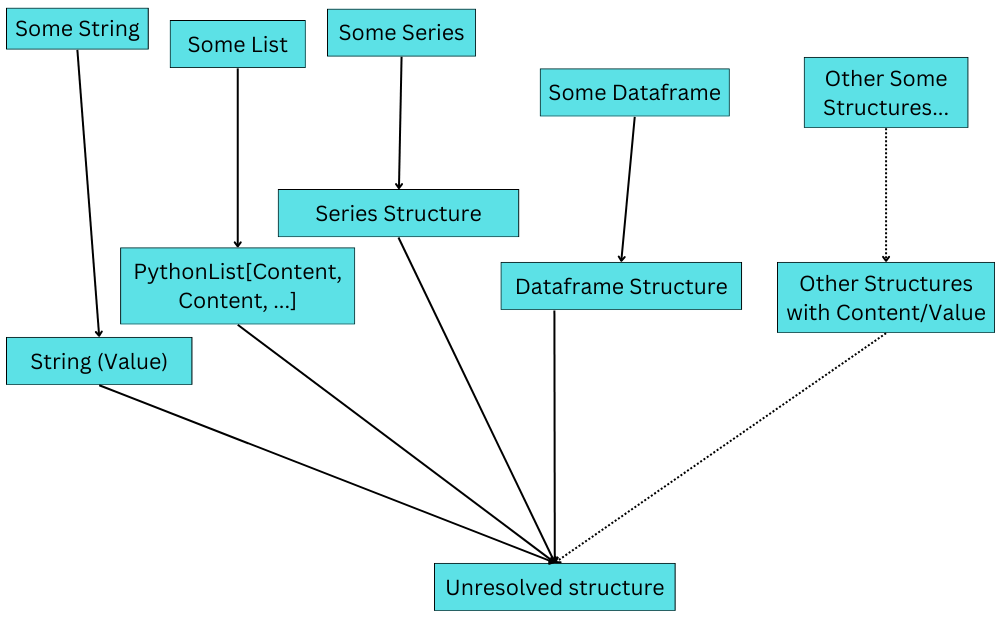
\includegraphics[scale=0.5]{img/Hierarchy}
\end{figure}

To satisfy the definition of a Lattice, every pair of elements must have a supremum and infimum.
It can be seen from the Figure~\ref{fig:abstract_hierarchy} that the infimum exists.
For two different values of the same type \verb|String("first")| and \verb|String("second")|, the infimum is
\verb|SomeString|.
For the two different types \verb|String("str")| and \verb(Int(7))|, the infimum is \verb|UnresolvedStructure|.
The other cases are analogous and are left as an exercise for the reader.

However, the idea misses suprema.
For that purpose we define another structure called \verb|NondeterministicStructure|.
The supremum of two elements of the hierarchy \verb|a| and \verb|b| is \verb|NondeterministicStructure(a, b)|.
The idea is also applicable recursively, so the value \\
\begin{verbatim}
NondeterministicStructure(
    NondeterministiStructure(
        SomeString,
        SomeInt
    ),
    SomeSeries
)
\end{verbatim}
is a valid element of the hierarchy.
The idea is shown in the Figure~\ref{fig:nondeterministic_structure}
With this idea, the hierarchy is finally a Lattice.
Note that it is not a Complete Lattice as the whole hierarchy does not have a supremum.

\begin{figure}[H]
    \caption{Nondeterministic structure}
    \label{fig:nondeterministic_structure}
    \centering
    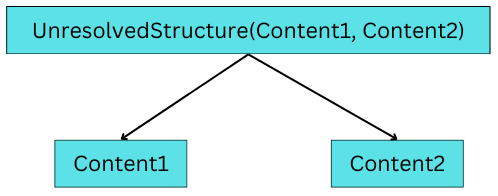
\includegraphics[scale=0.5]{img/unresolved_structure}
\end{figure}

The Nondeterministic Structure will mostly occur when there is a branching (e.g.~an if-statement) in the program, and we are not
able to resolve which branch we should go.
So the Nondeterministic Structure is a substitute that we need to use since we do not use the power set as the abstract
lattice anymore.


\section{Limitations}

The presented framework has some limitations that are important to discuss.
First, remembering just a Dataframe Structure prevents us from doing operations, that have the resulting Dataframe
Structure dependent on the values in a Dataframe.
Example of such operation can be the pivot operation.
The result of a pivot operation has columns named after values from a selected column.
But we do not know these values, since we only remember the Dataframe Structure.
Another example of an operation, that we are unable to resolve the resulting Dataframe of is a transpose.
The transpose function flips the whole dataframe along the diagonal (like with matrices), so the columns of the result
will be the rows of the original Dataframe and the column names of the result will be the index values of the original.
But, again, we do not know the index values.
In such situation there is no other option then just returning Some Dataframe.

Another possible problem can be an unknown value propagation, meaning that when there is a value with any uncertainty
(e.g.\ Nondeterministic Structure or Some value), using this value in an operation will in most cases lead to an
operation result with an uncertainty as well.

\section*{Summary}
\addcontentsline{toc}{section}{Summary}

\xxx{TODO :)}